\documentclass[11pt]{article}

\usepackage[margin=1in]{geometry}
\usepackage{amsmath,amssymb}
\usepackage{booktabs}
\usepackage{graphicx}
\usepackage{xcolor}
\usepackage{tikz}
\usetikzlibrary{arrows.meta,positioning,fit,backgrounds}
\usepackage[colorlinks=true,linkcolor=blue!50!black,urlcolor=blue!50!black]{hyperref}

\definecolor{seasonal}{RGB}{31,119,180}
\definecolor{arima}{RGB}{214,39,40}
\definecolor{rf}{RGB}{44,160,44}
\definecolor{varc}{RGB}{148,103,189}

\newcommand{\code}[1]{\texttt{\small #1}}

\title{\vspace{-1.5em}The \code{mstl\_multistep} Champion Model\\[0.3em]
\large MSTL $\rightarrow$ ARIMA $\rightarrow$ Random-Forest Residual,\\
with a Location--Scale Variance Head}
\author{Model configuration: \code{config\_arima012\_bank}}
\date{\today}

\begin{document}
\maketitle
\vspace{-1.5em}

\begin{abstract}
\noindent
This document describes the champion forecasting model in the \code{mstl\_multistep}
project: a CHAP-compatible monthly disease-case forecaster. It is an \emph{additive
decomposition} model on the log scale. Multiple Seasonal--Trend decomposition (MSTL)
removes the annual cycle; a \textbf{shared fixed-order ARIMA$(0,1,2)$} (the same order for
every location) models the deseasonalised dynamics \emph{and} supplies the predictive
spread; a Random Forest corrects the ARIMA residual using lagged climate anomalies, an
\textbf{expanded bank of indoor-residual-spraying (IRS) features} (incl.\ per-chemical decay
channels), and lagged self-history; and a \emph{location--scale variance head} widens the
predictive interval by the Random Forest's own uncertainty. On the frozen evaluation harness
(406 locations, 3-month horizon) it reaches a log-CRPS of \textbf{0.3123} and CRPS of
\textbf{81.88} --- a $\sim$4\% log-CRPS improvement over the climate-only baseline.
\end{abstract}

\section{Overview}

The model forecasts monthly disease cases $y_{\ell,t}$ for each location $\ell$. It works
entirely in $\log 1p$ space, $L_{\ell,t}=\log(1+y_{\ell,t})$, and writes that signal as a
sum of three estimated components plus noise:
\begin{equation}
L_{\ell,t} \;=\; \underbrace{S_{\ell,t}}_{\text{seasonal (MSTL)}}
\;+\; \underbrace{A_{\ell,t}}_{\text{AR / trend (ARIMA)}}
\;+\; \underbrace{g(x_{\ell,t})}_{\text{covariate correction (RF)}}
\;+\; \varepsilon_{\ell,t}.
\label{eq:additive}
\end{equation}
Each component is fit by a different estimator chosen for what it is good at: MSTL for a
stable repeating seasonal shape, ARIMA for autoregressive persistence \emph{and} calibrated
uncertainty, and a Random Forest for nonlinear, climate- and intervention-driven anomalies
that the univariate ARIMA cannot see. The probabilistic forecast is Gaussian in $\log 1p$
space and is transformed back with $\exp m1$.

\begin{center}
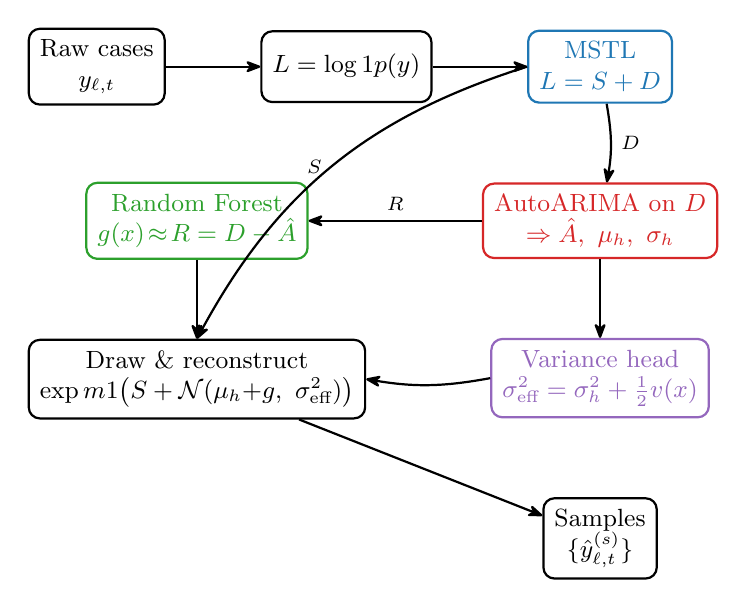
\begin{tikzpicture}[
  node distance=6mm and 12mm,
  box/.style={rounded corners,draw,thick,align=center,inner sep=4pt,minimum height=9mm,font=\small},
  >={Stealth[round]}, thick]

\node[box] (raw) {Raw cases\\$y_{\ell,t}$};
\node[box,right=of raw] (log) {$L=\log1p(y)$};
\node[box,seasonal,draw=seasonal,right=of log] (mstl) {MSTL\\$L=S+D$};

\node[box,arima,draw=arima,below=10mm of mstl] (arima) {AutoARIMA on $D$\\$\Rightarrow \hat A,\ \mu_h,\ \sigma_h$};
\node[box,rf,draw=rf,left=22mm of arima] (rf) {Random Forest\\$g(x)\!\approx\! R=D-\hat A$};
\node[box,varc,draw=varc,below=10mm of arima] (var) {Variance head\\$\sigma_{\text{eff}}^2=\sigma_h^2+\tfrac12 v(x)$};

\node[box,below=10mm of rf] (recon) {Draw \& reconstruct\\$\exp m1\big(S+\mathcal N(\mu_h{+}g,\ \sigma_{\text{eff}}^2)\big)$};
\node[box,below=10mm of var] (out) {Samples\\$\{\hat y^{(s)}_{\ell,t}\}$};

\draw[->] (raw)--(log);
\draw[->] (log)--(mstl);
\draw[->] (mstl) to[bend left=10] node[right,font=\scriptsize]{$D$} (arima);
\draw[->] (arima)-- node[above,font=\scriptsize]{$R$} (rf);
\draw[->] (arima)--(var);
\draw[->] (mstl.west) to[bend right=22] node[left,font=\scriptsize]{$S$} (recon.north);
\draw[->] (rf)--(recon);
\draw[->] (var.west) to[bend left=10] (recon.east);
\draw[->] (recon)--(out);
\end{tikzpicture}
\end{center}

\section{Data and notation}

Input is a CHAP-style monthly panel: one row per (location, month) with the target
\code{disease\_cases}, climate covariates, an IRS allocation column, and an admin
\code{district} id. There are 406 locations (sectors) over $2013$--$2026$.

\begin{center}
\small
\begin{tabular}{@{}ll@{}}
\toprule
Symbol & Meaning \\
\midrule
$y_{\ell,t}$ & disease cases at location $\ell$, month $t$ \\
$L_{\ell,t}=\log1p(y)$ & log-transformed target (modelling space) \\
$S_{\ell,t}$ & seasonal component (MSTL, period 12) \\
$D_{\ell,t}=L-S$ & deseasonalised series (trend $+$ remainder) \\
$\hat A_{\ell,t}$ & ARIMA in-sample fit of $D$; $\mu_h,\sigma_h$ its $h$-step forecast \\
$R_{\ell,t}=D-\hat A$ & ARIMA residual (the RF target) \\
$g(\cdot)$ & Random Forest mapping features $x$ to a residual correction \\
$v(x)$ & inter-tree variance of $g$ at $x$ (epistemic uncertainty) \\
\bottomrule
\end{tabular}
\end{center}

\section{Step 1 --- MSTL seasonal decomposition}

For each location independently, the $\log1p$ series is decomposed by MSTL into a seasonal
component (annual period $m=12$) and a deseasonalised remainder:
\[
L_{\ell,t} = S_{\ell,t} + D_{\ell,t}.
\]
$S$ captures the stable repeating within-year shape; $D=$ trend $+$ remainder is what the
rest of the pipeline forecasts. Into the forecast window the seasonal piece is extrapolated
\emph{seasonal-naive} (the last estimated annual cycle tiled forward). Series shorter than
two full seasons are treated as all-trend ($S\equiv 0$).

\begin{figure}[htbp]
\centering
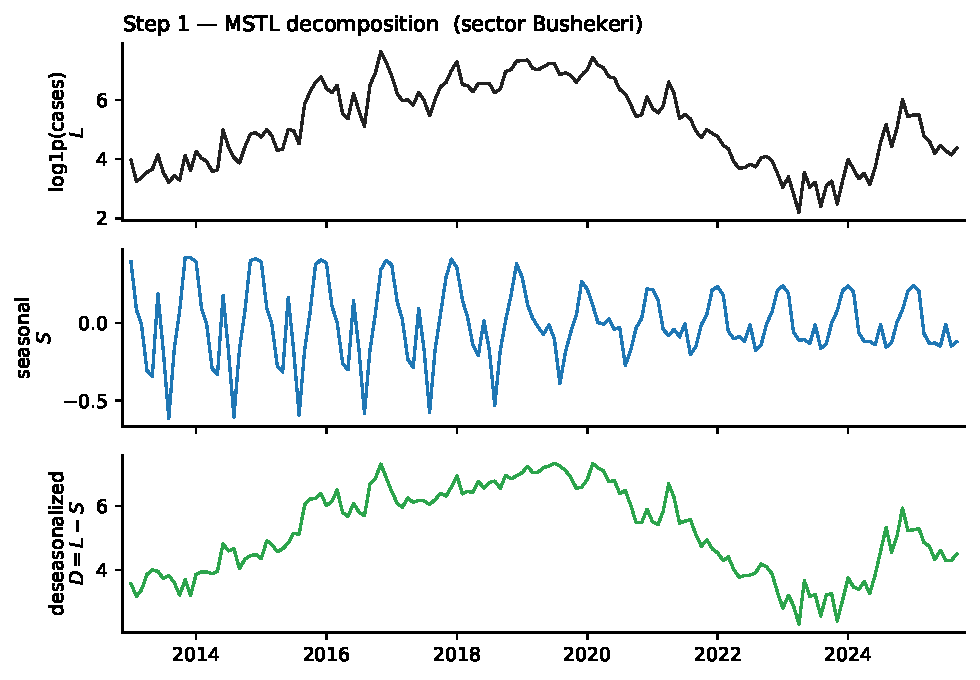
\includegraphics[width=\linewidth]{figs/fig1_decomposition.pdf}
\caption{Step 1 in action for one sector. The $\log1p$ case series $L$ (top) is split by MSTL
into a stable annual seasonal component $S$ (middle) and the deseasonalised series $D=L-S$
(bottom) that the rest of the pipeline forecasts.}
\label{fig:decomp}
\end{figure}

\section{Step 2 --- Shared fixed-order ARIMA base (mean and spread)}

A separate ARIMA is fit per location to the deseasonalised series $D$ (with
\code{season\_length} $=1$, since seasonality is already removed), but \textbf{all locations
share the same fixed order, ARIMA$(0,1,2)$} --- only each location's coefficients are
estimated. This replaced per-location AutoARIMA order selection, which on short (157-month)
noisy series is itself a source of noise (AutoARIMA overfits high-order/drift picks); a single
robust order generalises better and was the largest single improvement found ($-2\%$ log-CRPS).
See \code{arima\_in\_model.pdf} and \code{arima011\_math.pdf} for the order analysis and the
SES interpretation. ARIMA plays two roles:
\begin{enumerate}
\item \textbf{Autoregressive mean.} The $h$-step forecast mean $\mu_{\ell,h}$ carries
      persistence/trend in $D$. Its in-sample one-step fit $\hat A$ defines the residual
      $R=D-\hat A$ that the Random Forest then models.
\item \textbf{Predictive spread.} The forecast interval at level $68\%$ is converted to a
      Gaussian standard deviation $\sigma_{\ell,h}=(\text{hi}-\text{lo})/(2z)$. This
      $\sigma_h$ \emph{grows with horizon} and is the model's principal source of forecast
      uncertainty.
\end{enumerate}
A degenerate series (no finite history) falls back to a constant-mean / sample-sd baseline.

\section{Step 3 --- Random-Forest residual correction}

A single \emph{pooled} Random Forest $g$ is trained across all locations to predict the
ARIMA residual $R_{\ell,t}$ from a feature vector $x_{\ell,t}$. It is a deterministic
\emph{point} correction --- it nudges the mean, exploiting nonlinear structure ARIMA misses.
The feature vector combines four blocks:

\begin{enumerate}
\item \textbf{Lagged climate anomalies.} The three climate covariates are first
      MSTL-deseasonalised (so the model sees \emph{anomalies} relative to each one's own
      seasonal cycle), then lagged with \emph{per-covariate} windows reflecting the
      physical delay from weather to transmission:
      \begin{center}\small
      \begin{tabular}{@{}lc@{}}
      \toprule
      covariate & lags (months) \\ \midrule
      \code{rainfall\_era5} & $1\text{--}6$ \\
      \code{relative\_humidity} & $1\text{--}4$ \\
      \code{mean\_temperature} & $1\text{--}2$ \\
      \bottomrule
      \end{tabular}
      \end{center}
      Moisture-driven drivers (rain, humidity) get longer windows than temperature.

\item \textbf{Engineered IRS feature bank.} The raw \code{irs\_allocated} column is a sparse
      $0$--$1$ coverage fraction firing only in campaign months ($\sim$2.5\% of rows); its
      protective effect persists and is \emph{known in advance}, so it is expanded into a
      bank of dense, contemporaneous (lag-0) signals and the forest selects what matters:
      \begin{itemize}
      \item \code{level}, \code{since} (months since last campaign, capped),
            \code{cumulative} (campaign-count stock);
      \item \textbf{per-chemical decay channels} --- the geometric-decay protection split into
            \code{decay\_\{carbamate,pyrethroid,organophosphate,clothianidin\}}, each non-zero
            only while that insecticide class is the active one (from \code{irs\_insecticide\_used}),
            so the RF learns each chemical's effect magnitude (organophosphate/clothianidin
            strongest; pyrethroid near-dead, consistent with resistance);
      \item \textbf{decay basis} \code{decay2}, \code{decay8} (half-lives 2 and 8 months);
      \item \textbf{recency} flags \code{recent3/6/12} and \code{rounds12} (campaigns in the
            trailing year).
      \end{itemize}
      (The earlier 4-feature set \code{level/decay/since/cumulative} with a fixed 4-month decay
      was the prior champion; the bank improved on it.)

\item \textbf{Self-history (target lags).} The deseasonalised target $D$ lagged $1$--$3$
      months. In the forecast window, lags that fall ahead of the origin are
      \emph{bridged} with the ARIMA mean forecast $\mu_h$ (a non-recursive bridge), letting
      the RF pick up residual autocorrelation the linear ARIMA leaves behind.

\item \textbf{Location identity.} One-hot location dummies, so the pooled forest can retain
      per-series level/behaviour.
\end{enumerate}

\section{Step 4 --- Location--scale variance head}

The Random Forest correction is added as a point, so on its own it injects no uncertainty.
The variance head restores that: the forest's \textbf{inter-tree variance}
$v(x)=\operatorname{Var}_{\text{trees}} g(x)$ --- how much the 200 trees disagree --- is an
estimate of the correction's uncertainty, and it is folded into the predictive spread in
quadrature:
\begin{equation}
\sigma_{\text{eff},\ell,h}^2 \;=\; \sigma_{\ell,h}^2 \;+\; \kappa\, v(x_{\ell,h}),
\qquad \kappa = 0.5 .
\label{eq:varhead}
\end{equation}
This is the honest predictive variance ``total $=$ ARIMA forecast variance $+$ variance of
the mean correction.'' It corrects a mild under-dispersion and improves \emph{both} log-CRPS
and CRPS --- a rare non-trade-off in this project. (It is the productive form of an
EM/coordinate-descent idea: a mean-backfitting EM was a documented negative because it
reshuffled mean variance; moving the descent to the \emph{spread} coordinate is what worked.)

\begin{figure}[htbp]
\centering
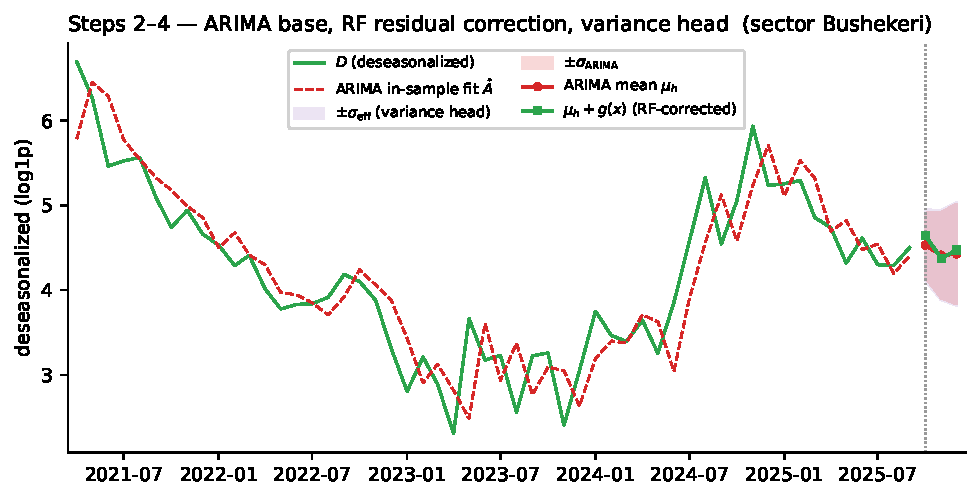
\includegraphics[width=\linewidth]{figs/fig2_arima_rf.pdf}
\caption{Steps 2--4 for the same sector, zoomed on the forecast origin (dotted line).
The ARIMA fits the deseasonalised series $D$ in-sample ($\hat A$, dashed) and forecasts the
mean $\mu_h$ with spread $\sigma_{\mathrm{ARIMA}}$; the Random Forest shifts the mean by the
correction $g(x)$ (green markers); the variance head widens the predictive spread from
$\sigma_{\mathrm{ARIMA}}$ to $\sigma_{\mathrm{eff}}$ (purple band). (Figures 1--3 illustrate the
shared pipeline; they were rendered on an immediately-prior champion config --- the structure
is identical.)}
\label{fig:arimarf}
\end{figure}

\section{Step 5 --- Reconstruction and sampling}

For each location and horizon step $h$, the forecast distribution in $\log1p$ space is
Gaussian, centred on seasonal $+$ ARIMA mean $+$ RF correction, with the widened spread:
\begin{equation}
\hat L_{\ell,h}^{(s)} \;=\; S_{\ell,h} \;+\; \mu_{\ell,h} \;+\; g(x_{\ell,h})
\;+\; \eta^{(s)},\qquad \eta^{(s)}\sim\mathcal N\!\big(0,\ \sigma_{\text{eff},\ell,h}^2\big),
\end{equation}
drawn $s=1,\dots,100$ times. Samples are mapped back to the count scale and clipped at zero:
\[
\hat y_{\ell,h}^{(s)} \;=\; \max\!\big(0,\ \exp m1(\hat L_{\ell,h}^{(s)})\big).
\]
The $100$ samples per (location, month) are the model's probabilistic forecast, scored by
log-CRPS (primary) and CRPS.

\begin{figure}[htbp]
\centering
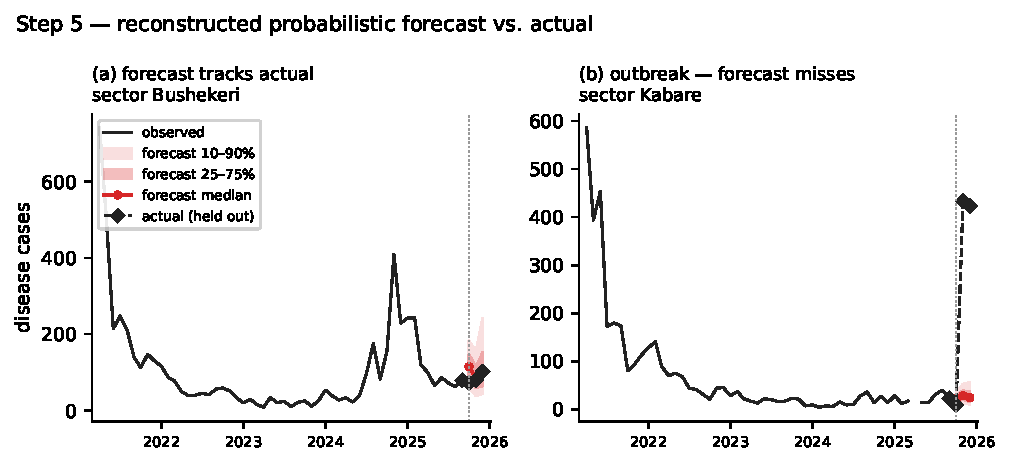
\includegraphics[width=\linewidth]{figs/fig3_forecast.pdf}
\caption{Step 5 on the count scale, for two sectors. \textbf{(a)} In a typical month the
reconstructed forecast (median, with $10$--$90\%$ and $25$--$75\%$ bands) tracks the held-out
actual. \textbf{(b)} For an explosive outbreak (actual ${\approx}7\times$ the $90\%$ band) the
model under-predicts: it captures climate- and season-driven dynamics but not idiosyncratic
outbreaks, which are the dominant remaining source of error and the reason the variance head
(which widens the interval where the forest is unsure) helps but cannot fully cover the tail.}
\label{fig:forecast}
\end{figure}

\section{Champion configuration}

\begin{center}
\small
\begin{tabular}{@{}lll@{}}
\toprule
Group & Setting & Value \\
\midrule
Transform & \code{log\_transform} & true ($\log1p$) \\
          & \code{season\_length\_monthly} & 12 \\
Base model & \code{prob\_model} & \code{rf\_residual} \\
           & \code{arima\_order} & \textbf{[0, 1, 2]} (shared, all locations) \\
           & \code{arima\_level} & 68 \\
Climate lags & \code{rainfall\_era5} & $1$--$6$ \\
             & \code{relative\_humidity} & $1$--$4$ \\
             & \code{mean\_temperature} & $1$--$2$ \\
             & \code{deseasonalize\_covariates} & all three \\
IRS & \code{irs\_column} & \code{irs\_allocated} \\
    & \code{irs\_chemical\_column} & \code{irs\_insecticide\_used} \\
    & \code{irs\_features} (bank) & level, since, cumulative, chem\_channels, \\
    & & decay2, decay8, recent3/6/12, rounds12 \\
Self-history & \code{rf\_target\_lags} & 3 \\
Variance head & \code{residual\_variance} & \code{tree} \\
              & \code{residual\_variance\_scale} ($\kappa$) & 0.5 \\
Random Forest & \code{n\_estimators} & 200 \\
              & \code{max\_depth} & none \\
              & \code{min\_samples\_leaf} & 3 \\
              & \code{max\_features} & sqrt \\
Sampling & \code{n\_samples} & 100 \\
\bottomrule
\end{tabular}
\end{center}

\section{Performance and design notes}

On the frozen main harness --- 406 locations, monthly, 3-month horizon, 12 backtest splits,
stride 1 --- the champion scores:
\begin{center}
\small
\begin{tabular}{@{}lcc@{}}
\toprule
Model & log-CRPS $\downarrow$ & CRPS $\downarrow$ \\
\midrule
Climate-only baseline (no IRS) & 0.3253 & 83.6 \\
$+$ IRS features, per-covariate lags, leaf$=3$, target lags & 0.3203 & 82.97 \\
$+$ variance head (\code{config\_tgtlag3\_var}) & 0.3200 & 82.88 \\
$+$ shared ARIMA$(0,1,2)$ order (\code{config\_arima012}) & 0.3135 & 81.77 \\
$+$ IRS feature bank \;\textbf{(champion, \code{config\_arima012\_bank})} & \textbf{0.3123} & \textbf{81.88} \\
\bottomrule
\end{tabular}
\end{center}

\noindent\textbf{What drives the model's accuracy.} The largest single lever was switching
from per-location AutoARIMA \emph{order selection} to one \textbf{shared fixed ARIMA$(0,1,2)$}
order ($-2\%$ log-CRPS): order selection on short noisy series is itself noise. On top of that,
the levers that helped all either \emph{add information} (the IRS feature bank incl.\ per-chemical
channels; lagged self-history) or \emph{account for uncertainty honestly} (the variance head).
A long list of alternatives --- EM/backfitting on the mean, Fourier seasonal features, $\sigma$
rescaling, quantile-GBM residuals, horizon-scaled variance, vegetation indices, spatial
(same-district) neighbour features, chemical-\emph{rate} decay, and reduced location encodings
(district/cluster) --- were tested and did not help. The recurring lesson: let each component
own what it is best at (MSTL the season, ARIMA the persistence \emph{and the spread}, the forest
the nonlinear anomalies), prefer one robust shared configuration over per-series selection on
short data, add information rather than re-shuffle it, and account for every component's
uncertainty honestly.

\end{document}
